\documentclass[12pt]{article}
\usepackage{graphicx}
\usepackage{amsmath}
\usepackage{placeins}

\begin{document}

\begin{titlepage}
    \begin{center}
        \huge
        Chebyschev IIR\\Filter Design Report
        \vfill
        \large
        Student Details:\\\vspace{3pt}
        Name: Kanak Yadav\\\vspace{3pt}
        Roll No: 20D070044\\\vspace{3pt}
        Filter Number: 55\\\vspace{3pt}
        Group Number: 37\\\vspace{60pt}
        Reviewer Details:\\\vspace{3pt}
        Name: Pal Abhijeet Manoj\\\vspace{3pt}
        Roll No: 200100107
        \vfill
    \end{center}
\end{titlepage}

\section{Design}
\subsection{Un-normalized Discrete Time Filter}
The un-normalized discrete time filter specifications are uniquely assigned to each student using the filter number assigned to them.

The Chebyschev filter to be designed is a Bandstop filter for filter numbers 1 to 80 and a Bandpass filter for filter numbers 81 to 160.

Hence, we would be designing a Chebyschev IIR Bandstop Filter.

The stopband for the Bandstop filter is BL(m) kHz to BH(m) kHz, which are defined as:
\[q(m) = r(m) = 5\]
\begin{align*}
    BL(m) &= 20 + 3 q(m) + 11 r(m),\\
    &= 20 + 3(5) + 11(5)\\
    &= 90,\\
    BH(m) &= BL(m) + 40,\\
    &= 90 + 40\\
    &= 130.
\end{align*}
Therefore, the stopband edges are:
\begin{align*}
    f_{s1} &= 90 kHz,\\
    f_{s2} &= 130 kHz.
\end{align*}
The transition band width is given to be\[\Delta_f = 5 kHz.\]
Therefore, the passband edges are:
\begin{align*}
    f_{p1} &= f_{s1} - \Delta_f = 85 kHz,\\
    f_{p2} &= f_{s2} + \Delta_f = 135 kHz.
\end{align*}

Now we can state the specifications of the discrete-time Bandstop filter.
\newpage
\hline
\vspace{10pt}
\textbf{Specifications:}
\begin{itemize}
    \item Passband: 0 to 85 kHz and 135 kHz to 212.5 kHz (since $f_s$ = 425 kHz),
    \item Stopband: 100 kHz to 175 kHz,
    \item Passband and Stopband tolerance: 0.15,
    \item Passband and Stopband nature: Equiripple and Monotonic respectively.
\end{itemize}
\hline

\subsection{Normalized Digital Filter}
For normalizing the frequencies, we need to make the sampling frequency map to $2\pi$. Thus,
\[\omega = \frac{2\pi f}{f_s}\]

This gives us the normalized digital frequencies as follows:
\begin{table}[h]
    \centering
    \begin{tabular}{|c|c|}\hline
         Discrete time frequency&Normalized digital frequency\\
         $f$ (kHz)&$\omega$ (radians)\\\hline
         0&0\\\hline
         85&$\omega_{p1}$ = 1.2566371\\\hline
         90&$\omega_{s1}$ = 1.3305569\\\hline
         130&$\omega_{s2}$ = 1.9219155\\\hline
         135&$\omega_{p2}$ = 1.9958353\\\hline
         212.5&$\pi$\\\hline
    \end{tabular}
    \caption{Normalizing frequency.}
    \label{tab:1}
\end{table}

Now we can state the specifications of the digital Bandstop filter.
\newline
\hline
\vspace{10pt}
\textbf{Specifications:}
\begin{itemize}
    \item Passband: 0 to 1.2566371 and 1.9958353 to  $\pi$,
    \item Stopband: 1.3305569 to 1.9219155,
    \item Passband and Stopband tolerance: 0.15,
    \item Passband and Stopband nature: Equiripple and Monotonic respectively.
\end{itemize}
\hline

\subsection{Analog Bandstop Filter}
For converting the normalized digital specifications to the specifications for an analog filter of the same type (Bandstop), we use the bilinear transformation:
\[\Omega &= \tan(\omega/2)\]
This gives us the analog Bandstop frequencies as:
\begin{table}[h]
    \centering
    \begin{tabular}{|c|c|}\hline
         Normalized digital frequency&Analog frequency\\
         $\omega$ (radians)&$\Omega$\\\hline
         0&0\\\hline
         1.2566371&$\Omega_{p1}$ = 0.7265425\\\hline
         1.3305569&$\Omega_{s1}$ = 0.7845976\\\hline
         1.9219155&$\Omega_{s2}$ = 1.4312732\\\hline
         1.9958353&$\Omega_{p2}$ = 1.5502977\\\hline
         $\pi$&$\infty$\\\hline
    \end{tabular}
    \caption{Applying the bilinear transformation.}
    \label{tab:2}
\end{table}

Now we can state the specifications of the digital Bandstop filter.
\newline
\hline
\vspace{10pt}
\textbf{Specifications:}
\begin{itemize}
    \item Passband: 0 to 0.7265425 and 1.5502977 to $\infty$,
    \item Stopband: 0.7845976 to 1.4312732,
    \item Passband and Stopband tolerance: 0.15,
    \item Passband and Stopband nature: Equiripple and Monotonic respectively.
\end{itemize}
\hline

\subsection{Frequency Transformation}
We need to employ a frequency transformation to convert our Bandstop filter specifications into those of a lowpass filter. For this, we use the frequency transformation derived from the impedance of a parallel LC circuit:
\[s_L = \frac{Bs}{s^2 + \Omega_0^2},\]
where the subscript L stands for Lowpass. $\Omega_0$ is the resonant frequency and B is the bandwidth of the parallel LC circuit. Substituting the values of s$_L$ and s, we get
\begin{align*}
    j\Omega_L &= \frac{B(j\Omega)}{(j\Omega)^2 + \Omega_0^2}\\
    &= j\frac{B\Omega}{(-\Omega^2 + \Omega_0^2)}\\
    \Omega_L &= \frac{B\Omega}{\Omega_0^2 - \Omega^2}
\end{align*}
Now, we have two degrees of freedom, $\Omega_0$ and B. We also decide to follow the convention that the passband edge of the lowpass filter, in both the positive and negative half of the $\Omega_L$ axis, has a magnitude of one. In other words, we want $\Omega_{p1}$ and $\Omega_{p2}$ to map to +1 and -1 respectively on the $\Omega_L$ axis. To achieve this, we solve the following two equations
\[+1 = \frac{B\Omega_{p1}}{\Omega_0^2 - \Omega_{p1}^2}\]
and
\[-1 = \frac{B\Omega_{p2}}{\Omega_0^2 - \Omega_{p2}^2}\]
Solving we get
\begin{align*}
    B &= \Omega_{p2} - \Omega_{p1}\\
    \Omega_0 &= \sqrt{\Omega_{p2}\Omega_{p1}}
\end{align*}
By substituting the value of $\Omega_{p1}$ and $\Omega_{p2}$, we get
\begin{align*}
    B &= 1.5502977 - 0.7265425 = 0.8237552\\
    \Omega_0 &= \sqrt{(1.5502977)(0.7265425)} = \sqrt{1.1263572} \approx 1.0612998
\end{align*}
\newpage
\hline
\vspace{10pt}
\textbf{Transformation and Parameters}
\begin{itemize}
    \item Transformation:\[\Omega_L = \frac{B\Omega}{\Omega_0^2 - \Omega^2}\]
    \item Parameters:
    \begin{itemize}
        \item $\Omega_0$ = 1.0612998,
        \item B = 0.8237552
    \end{itemize}
\end{itemize}
\hline

\subsection{Analog Lowpass Filter}
Substituting the values of $\Omega_o$ and B, we get the frequency transformation to be employed as:
\[\Omega_L = \frac{(0.8237552)\Omega}{(1.1263572) - \Omega^2}\]
This gives us the analog lowpass frequencies as:
\begin{table}[!h]
    \centering
    \begin{tabular}{|c|c|}\hline
         Analog frequency&Analog Lowpass Frequency\\
         $\Omega$ &$\Omega_L$\\\hline
         0$^+$&0$^+$\\\hline
         0.7265425&$\Omega_{Ls1}$ = 1.2653920\\\hline
         0.7845976&$\Omega_{Lp1}$ = 1\\\hline
         $\Omega_0^-$&$\infty^+$\\\hline
         $\Omega_0^+$&$\infty^-$\\\hline
         1.4312732&$\Omega_{Lp2}$ = -1\\\hline
         1.5502977&$\Omega_{Ls2}$ = -1.2785044\\\hline
         $\infty$&$0$^-$$\\\hline
    \end{tabular}
    \caption{Analog frequency transformation.}
    \label{tab:3}
\end{table}

The passband edge of the lowpass filter was specified to be one while employing the frequency transformation but, the stopband edge now has two possible values of which, we choose the more stringent value (the value with a smaller magnitude) since satisfying the stronger specifications will automatically satisfy the weaker specifications. Thus
\begin{align*}
    \Omega_p &= 1\\
    \Omega_s &= min(abs(\Omega_{Ls1}), abs(\Omega_{Ls1}))\\
    &= min(1.2653920, 1.2785044)\\
    \Omega_s &= 1.2653920
\end{align*}

Now we can state the specifications of the analog lowpass filter.
\newline
\hline
\vspace{10pt}
\textbf{Specifications:}
\begin{itemize}
    \item Passband: 0 to 1,
    \item Stopband: 1.2653920 to  $\infty$,
    \item Passband and Stopband tolerance: 0.15,
    \item Passband and Stopband nature: Equiripple and Monotonic respectively.
\end{itemize}
\hline

\subsection{Chebyschev Analog Lowpass Transfer Function}
The Chebyschev analog lowpass transfer function is given as:
\[\text{H}_{\text{analog, LPF}}\text{(s}_\text{L}\text{)} = \frac{C}{\prod_{k\epsilon LHP}(s - s_k)}.\]
N is given by the specifications as:
\[N \geq \frac{\cosh^{-1}\sqrt{\frac{D_2}{D_1}}}{\cosh^{-1}{\frac{\Omega_s}{\Omega_p}}},\]
where $D_1$ and $D_2$ are given by:
\begin{align*}
    D_1 &= \frac{1}{(1 - \delta_1)^2} - 1,\\
    D_2 &= \frac{1}{\delta_2^2} - 1.
\end{align*}
$\delta_1$ and $\delta_2$ are the passband and stopband tolerances.
\begin{align*}
    D_1 &= \frac{1}{(1 - 0.15)^2} - 1 = 0.3840830\\
    D_2 &= \frac{1}{0.15^2} - 1 = 43.444444
\end{align*}
This gives us
\[N \geq \frac{\cosh^{-1}(\sqrt{113.11211})}{\cosh^{-1}(1.1430597)} \approx 4.2829034,\]
Hence, we choose\[N = 5.\]
Since N is odd,
\[C = \prod_{k\epsilon LHP}|s_k|\]
to satisfy,
\[|\text{H}_{\text{analog, LPF}}\text{(0)}| = 1,\]
since for odd N,
\[C_N(0) = 0.\]
Now the poles can be found by setting the denominator of the magnitude squared form of the Chebyschev lowpass filter transfer function to zero.
\[|\text{H}_{\text{analog, LPF}}\text{(s}_\text{L}\text{)}|^2 = \frac{1}{1 + \epsilon^2C_N^2(\frac{s}{j\Omega_p})}\]
where,
\[\epsilon = \sqrt{D_1} = 0.6197443.\]
Now,
\[1 + \epsilon^2C_N^2\left(\frac{s_k}{j\Omega_p}\right) = 0\]
\[C_N^2\left(\frac{s_k}{j\Omega_p}\right) = \frac{-1}{\epsilon^2}\]
\[C_N\left(\frac{s_k}{j\Omega_p}\right) = \pm\frac{j}{\epsilon}\]

To solve this, let us take
\[\cos^{-1}(\left\frac{s_k}{j\Omega_p}\right) = A_k + jB_k\]
\[\frac{s_k}{j\Omega_p} = \cos(A_k + jB_k)\]
\[s_k = j\Omega_p(cos(A_k)cos(jB_k) - sin(A_k)sin(jB_k))\]
\[s_k = \Omega_psin(A_k)sinh(B_k) + j\Omega_pcos(A_k)cosh(B_k)\]
It is interesting to see that while the poles of the Butterworth lowpass filter transfer function lie on the circle with magnitude $\omega_c$, the poles of the Chebyschev lowpass filter transfer function lie on an ellipse with the imaginary axis as its major axis. The equation of the ellipse is given by,
\[\left(\frac{\Sigma_k}{\Omega_psinh(B_k)}\right)^2 + \left(\frac{\Omega_k}{\Omega_pcosh(B_k)}\right)^2 = 1,\]
where,
\[s_k = \Sigma_k + j\Omega_k.\]
Now, substituting this, to find $A_k$ and $B_k$,
\[cos(NA_k+jNB_k) = \pm\frac{j}{\epsilon}\]
\[cos(NA_K)cos(jNB_k) - sin(NA_k)sin(jNB_k) = \pm\frac{j}{\epsilon}\]
\[cos(NA_K)cosh(NB_k) - jsin(NA_k)sinh(NB_k) = \pm\frac{j}{\epsilon}\]
By comparing the real and imaginary parts on both sides we get,
\[cos(NA_K)cosh(NB_k) = 0 \implies cos(NA_k) = 0\]
\[A_k = \frac{\pi}{2N} + \frac{k\pi}{N}.\]
And,
\[sin(NA_k)sinh(NB_k) = \frac{1}{\epsilon} \implies sinh(NB_k) = \frac{1}{\epsilon}\]
\[B_k = \frac{1}{N}sinh^{-1}(\frac{1}{\epsilon})\]
\[B_k = 0.2512306\]
Now, we can take any sign for the square root provided that we vary k over 2N contiguous integers and get the poles as:
\[s_k = \Omega_psin(A_k)sinh(B_k) + j\Omega_pcos(A_k)cosh(B_k)\]
To obtain the LHP (Left Half Plane) poles with the positive square root taken, we need to take the values of k ranging from N to 2N-1.

Now we can find the Chebyschev analog lowpass filter transfer function.
\textbf{$\text{H}_{\text{analog, LPF}}\text{(s}_\text{L}\text{)}$:}
\begin{figure}[h]
    \centering
    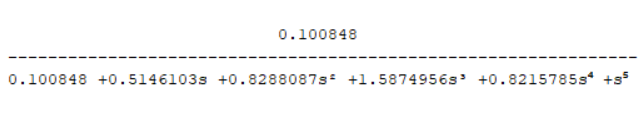
\includegraphics[width=\textwidth]{h_analog_lowpass.png}
    \caption{Screenshot from SCILAB Console.}
\end{figure}

\subsection{Analog Bandstop Transfer Function}
This can be obtained by replacing s$_\text{L}$ with F(s), the frequency transformation that we had employed earlier:
\[s_L \leftarrow F(s) = \frac{Bs}{s^2 + \Omega_0^2}\]
\textbf{H$_{\text{analog, BSF}}\text{(s)}$}
\begin{figure}[h]
    \centering
    \includegraphics[width=\textwidth]{h_analog_Bandstop.png}
    \caption{Screenshot from SCILAB Console.}
\end{figure}

\subsection{Discrete Time Bandstop Transfer Function}
This can be obtained by applying the bilinear transformation to s:
\[s \leftarrow \frac{1 - z^{-1}}{1 + z^{-1}}\]
\textbf{H$_{\text{discrete time, BSF}}\text{(z)}$}
\begin{figure}[h]
    \centering
    \includegraphics[width=\textwidth]{h_discrete_time_Bandstop.png}
    \caption{Screenshot from SCILAB Console.}
\end{figure}

\section{Review}
I have reviewed Abhijeet's report and certify it to be correct.

\section{Plots}
Here are some plots generated using SCILAB:
\begin{figure}[!h]
    \centering
    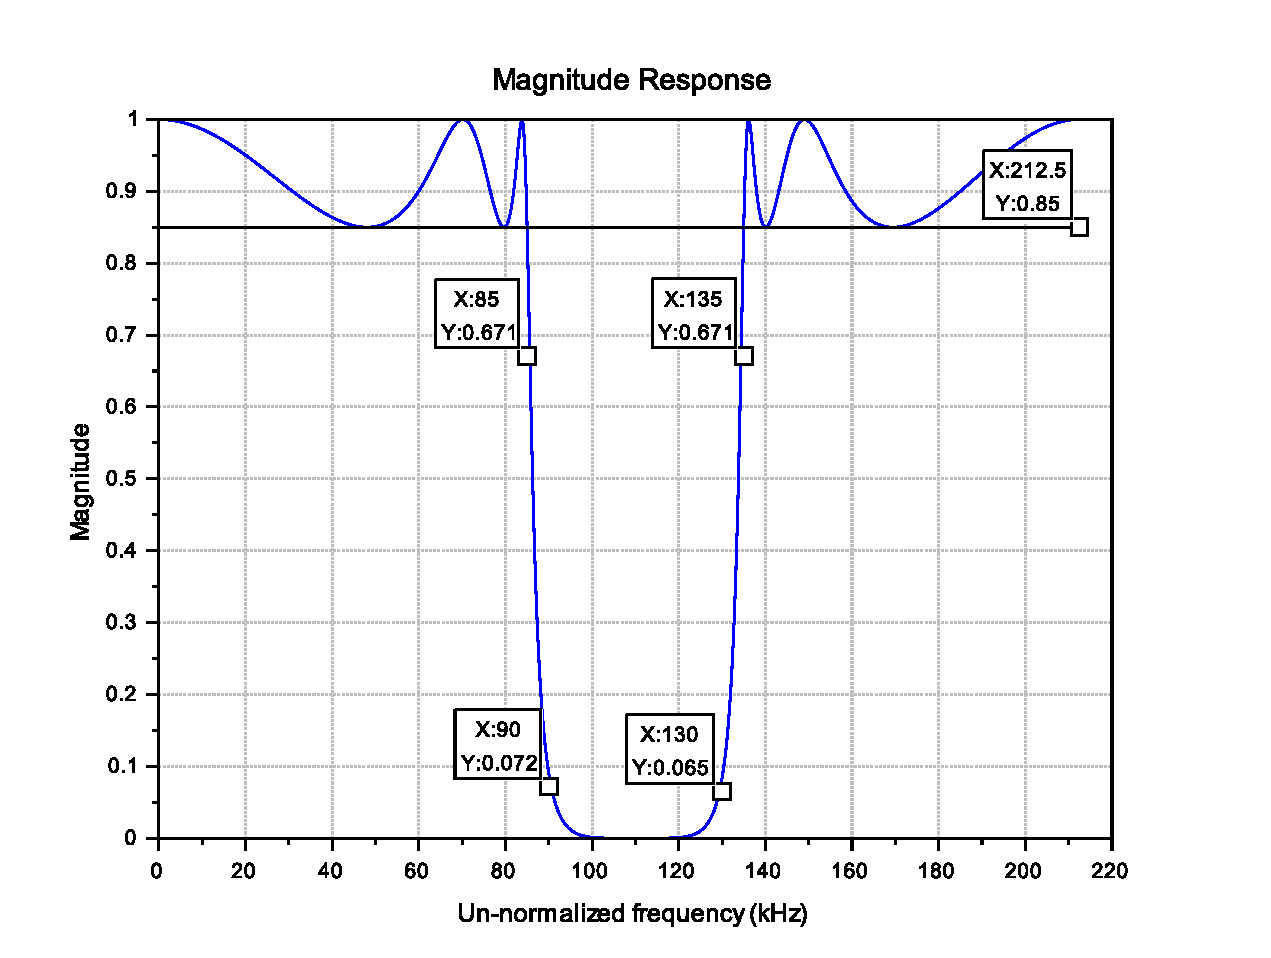
\includegraphics[scale=0.6]{mag.pdf}
    \quad
    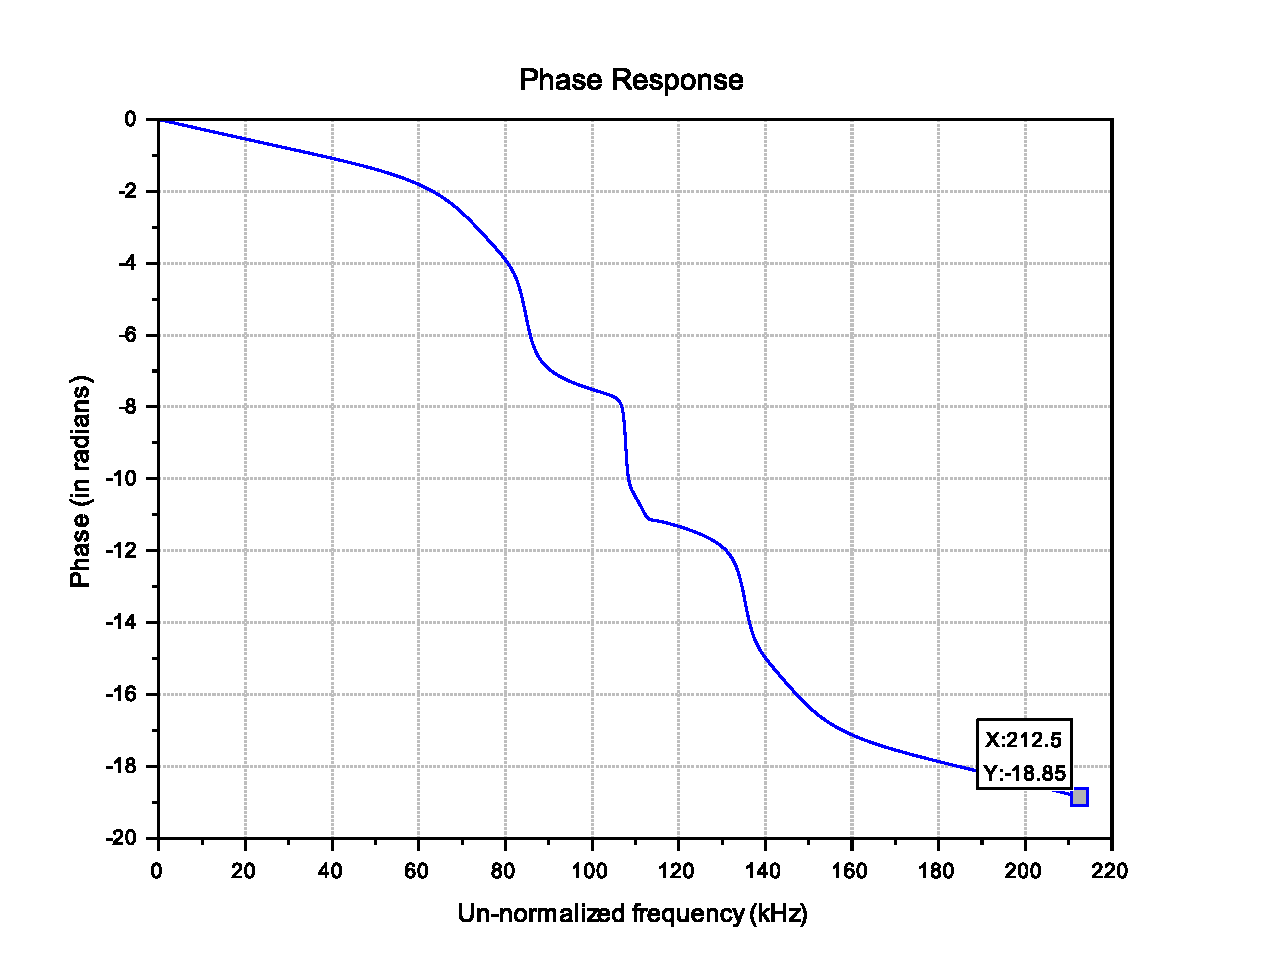
\includegraphics[scale=0.6]{phase.pdf}
\end{figure}
\begin{figure}[!h]
    \centering
    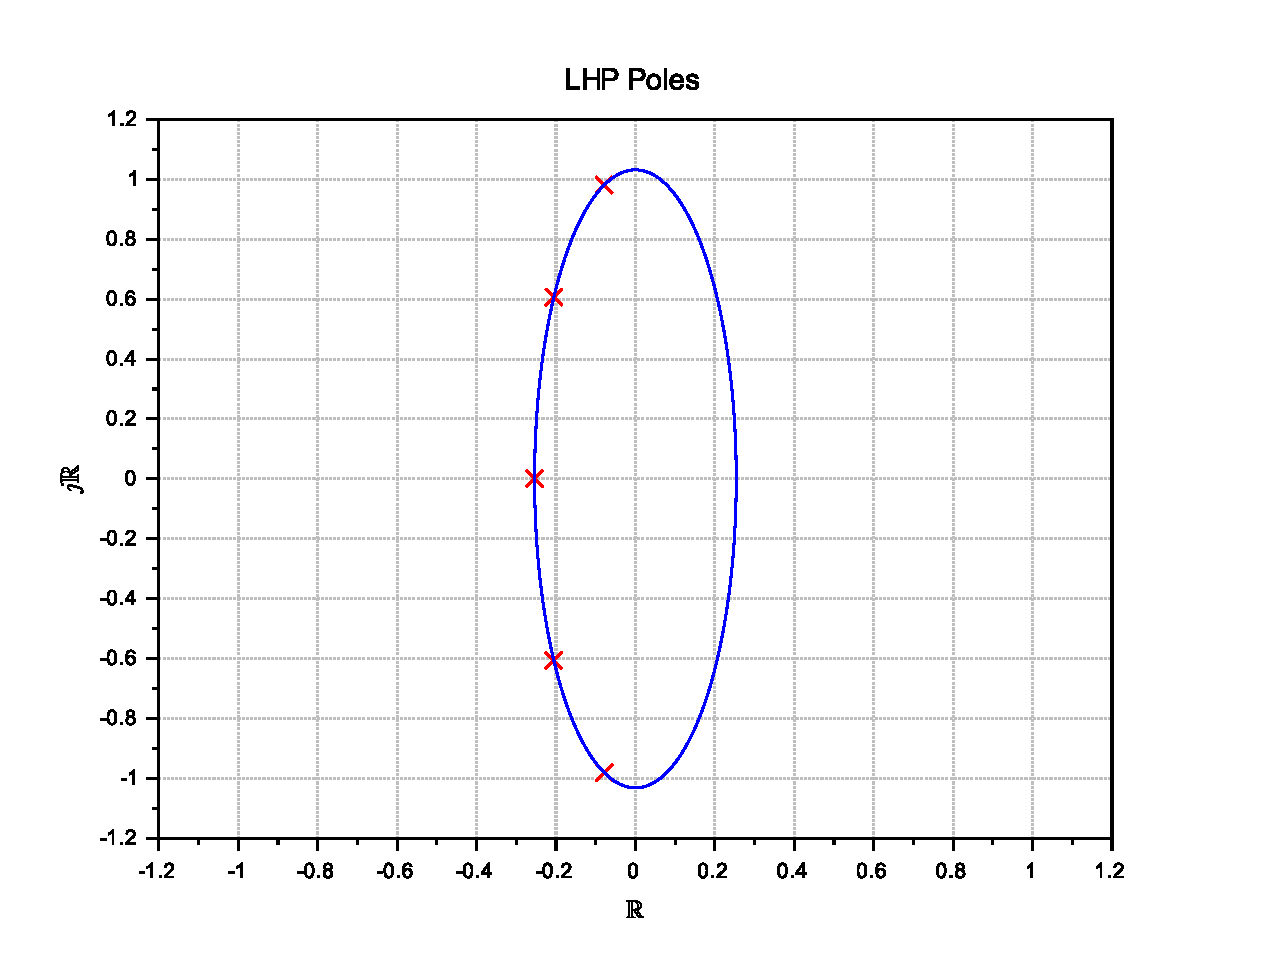
\includegraphics[scale=0.6]{poles.pdf}
    \caption{Poles of the Chebyschev lowpass transfer function.}
\end{figure}

\end{document}
